% =====================================================================
%  重复控制器周期在线自整定（锁相极值搜索）—— 算法、原理与实验
%  编译：xelatex 两遍（MiKTeX + ctex）
%  版本：2026-11-11 晚（含锁相 ESC 实测结果）
% =====================================================================
\documentclass[UTF8,fontset=windows,a4paper,11pt]{ctexart}

\usepackage{amsmath,amssymb,amsthm,mathtools}
\usepackage{booktabs,array}
\usepackage{graphicx}
\usepackage{float}
\usepackage{geometry}
\geometry{left=2.6cm,right=2.6cm,top=2.6cm,bottom=2.6cm}
\usepackage{xcolor}
\usepackage{tikz}
\usetikzlibrary{positioning,arrows.meta}
\usepackage[hidelinks]{hyperref}
\allowdisplaybreaks

\newtheorem{proposition}{命题}
\newtheorem{assumption}{假设}
\newtheorem{theorem}{定理}
\newtheorem{lemma}{引理}
\newtheorem{corollary}{推论}
\newtheorem{remark}{注}

\newcommand{\clip}{\operatorname{clip}}
\newcommand{\sgn}{\operatorname{sgn}}
\newcommand{\Tg}{T_{\mathrm{gross}}}

\title{\bfseries 重复控制器周期在线自整定：\\
基于基波幅值锁相极值搜索的双层自适应算法}
\author{技术报告}
\date{2026 年 11 月 11 日}

\begin{document}
\maketitle

\begin{abstract}
重复控制（RC）的内模周期若与扰动周期失配，其窄带陷波将失谐，周期扰动抑制能力急剧下降。
本文在既有 $T=2\pi/\omega$ 频率自适应之外，增加一层以“基波残余幅值 $A$”为目标的\textbf{锁相极值搜索}，
在线修正 $T=\Tg(1+\delta)$，从而同时对齐扰动的\textbf{频率}与\textbf{相位}。

主要结果：（1）$A$ 对周期失谐单调且灵敏（$1\%$ 周期误差约带来 $2.6\sim3.5\%$ 的 $A$ 变化），
可用作整定目标；（2）真实最优周期为 $\delta^{*}\approx-12\%$（$T=88$\,ms），
与记忆低通 $\tau=20$\,ms 带来的相位滞后（$51.5^{\circ}\Leftrightarrow14.3$\,ms）吻合，
并非标称的 $2\pi/\omega$；（3）锁相 ESC 从 $-5\%$ 出发 24\,s 内收敛至 $-8.1\%$，
稳态转速误差 RMS 由 $30.54$ 降至 $27.6\sim27.9$\,rpm（$-9\%\sim-10\%$），
与离线扫描最优（$27.56$\,rpm）相差不超过 $1.2\%$。

\vspace{4pt}
\noindent\textbf{关键词：}重复控制；自适应内模；极值搜索；锁相解调；PMSM
\end{abstract}

% ---------------------------------------------------------------------
\section{引言}

重复控制以“延迟一周期 + 正反馈”构造内模，在扰动频率及其整数倍处形成近似理想的陷波。
其性能高度依赖内模周期 $T$ 与真实扰动周期的匹配程度。工程上通常取 $T=2\pi/\omega$，
但该式只保证\textbf{频率}对齐，不保证\textbf{相位}对齐：记忆低通 $\tau$、控制拍离散化、
电流环与采样延时都会引入等效相移，使真实最优周期系统性偏离标称值。

本文在图~\ref{fig:arch} 的双层结构中，用基波残余幅值 $A$ 作为目标函数，
通过锁相极值搜索在线寻找最优 $\delta$。选 $A$ 而非宽带误差 RMS 的理由：
（1）$\pm10\%$ 带通使 $A$ 对非内模频段的振动与噪声免疫；
（2）$A$ 是单值、可跨工况比较的标量；（3）$A$ 对周期失谐单调且灵敏。

\begin{figure}[t]
\centering
\begin{tikzpicture}[>=Stealth,node distance=6mm,
  box/.style={draw,rounded corners=2pt,align=center,inner sep=4pt,minimum height=9mm},
  esc/.style={draw,dashed,rounded corners=2pt,align=center,inner sep=4pt,minimum height=9mm}]
\node[box] (eso) {ESO\\$\beta_1,\beta_2,G(e_1)$};
\node[box,right=10mm of eso] (rc) {重复通道\\$v+\tau\dot v=Qv(t-T)+\beta_3G(e_1)$};
\node[box,right=10mm of rc] (plant) {PMSM\\$J\dot\omega=K_ti_q^*-T_L(\theta)$};
\node[esc,below=10mm of rc] (bp) {带通 $\pm10\%$\\$Q_{\mathrm{bp}}=5$};
\node[esc,below=6mm of bp] (rms) {$A=\sqrt{\tfrac1{T}\int_{t-T}^{t}y_{\mathrm{bp}}^2}$};
\node[esc,below=6mm of rms] (escbox) {锁相 ESC\\$\hat\delta\leftarrow\hat\delta-\sigma\sgn(I)$};
\node[box,left=10mm of escbox] (tgen) {$\Tg=\dfrac{2\pi}{\omega_f}$\\$T=\Tg(1+\delta)$};
\draw[->] (plant.west) -- node[above,font=\scriptsize]{$\omega$} (rc.east);
\draw[->] (rc.west) -- (eso.east);
\draw[->] (eso.west) -- ++(-8mm,0) |- (tgen.north);
\draw[->] (plant.south) |- ++(0,-4mm) -| (bp.east);
\draw[->] (bp) -- (rms);
\draw[->] (rms) -- (escbox);
\draw[->] (escbox) -- (tgen);
\draw[->] (tgen.north) |- node[pos=0.75,left,font=\scriptsize]{$T$} (rc.north);
\end{tikzpicture}
\caption{双层自适应结构：内层 $T=2\pi/\omega$（频率对齐），外层锁相极值搜索修正 $\delta$（相位对齐）。}
\label{fig:arch}
\end{figure}

% ---------------------------------------------------------------------
\section{系统与既有结构}

\subsection{被控对象}
\begin{equation}
J_{\mathrm{dim}}\dot\omega=K_{t,\mathrm{dim}}i_q^*-T_L(\theta),\qquad \dot\theta=\omega ,
\end{equation}
\begin{equation}
T_L(\theta)=T_0+A_T\sum_{n=1}^{6}a_n\sin(n\theta)+T_{\mathrm{vib}}(t)+\varepsilon_T(t).
\end{equation}

\subsection{类 fal ESO}
\begin{align}
e_1&=\omega-z_1,\\
\dot z_1&=-\frac{B}{J_{\mathrm{dim}}}z_1+z_2+z_3+\frac{K_{t,\mathrm{dim}}}{J_{\mathrm{dim}}}i_q^*+\beta_1G(e_1),\\
\dot z_2&=\beta_2G(e_1),\qquad z_3=v,
\end{align}
\begin{equation}
G(e)=\Big(|e|+\delta_c\lambda^{-1/a}\Big)^{a}\tanh\!\Big(\frac{\lambda e}{\delta_c}\Big),
\qquad \beta_1=2\omega_o,\ \beta_2=\omega_o^2 .
\end{equation}

\subsection{重复通道}
\begin{equation}
\boxed{\;v(t)+\tau\dot v(t)=Q\,v(t-T)+\beta_3G(e_1)\;}
\label{eq:rc}
\end{equation}
离散形式（$\Delta t_s=1$\,ms）：
\begin{equation}
v[k]=v[k-1]+\frac{\Delta t_s}{\tau}\big(\chi[k]-v[k-1]\big),\qquad
\chi[k]=Q\,v[k-n_d]+\beta_3G(e_1[k]).
\end{equation}

% ---------------------------------------------------------------------
\section{周期失配的机理与灵敏度}

\subsection{陷波宽度}
\begin{equation}
\big|\mathcal{G}(f)\big|\ \propto\ \frac{1}{\big|1-Q\,e^{-j2\pi fT}\big|},
\end{equation}
令失配率 $\varepsilon=(T-T_0)/T_0$，在 $fT_0=1$ 处
\begin{equation}
\big|1-Qe^{-j2\pi\varepsilon}\big|\approx
\sqrt{(1-Q)^2+\big(2\pi Q\varepsilon\big)^2}.
\end{equation}

\begin{table}[h]
\centering
\caption{周期失配与内模等效增益衰减（$Q=0.98$）}
\begin{tabular}{@{}ccc@{}}
\toprule
周期误差 $\varepsilon$ & 相位误差 & 增益相对衰减 \\
\midrule
$0$      & $0^\circ$  & $1\times$ \\
$1\%$    & $3.6^\circ$& $3.3\times$ \\
$2\%$    & $7.2^\circ$& $6.3\times$ \\
$5\%$    & $18^\circ$ & $15\times$ \\
\bottomrule
\end{tabular}
\end{table}

陷波半宽
\begin{equation}
\Delta f_{\pm}=\frac{1-Q}{2\pi T}\approx 0.03\ \mathrm{Hz}\quad(\pm0.3\%).
\end{equation}

\subsection{相位对齐条件与理论最优周期}

把式 \eqref{eq:rc} 写成频域传递函数（$E$ 为输入、$V$ 为输出）：
\begin{equation}
\frac{V(s)}{E(s)}=\frac{\beta_3}{1+\tau s-Q\,e^{-sT}} .
\label{eq:rc_tf}
\end{equation}
重复通道对频率 $\omega$ 的扰动抑制能力由分母模长 $|D(j\omega)|$ 决定，$|D|$ 越小增益越大。
记 $\theta=\omega T$，则
\begin{equation}
\big|D(j\omega)\big|^2=\big|1+j\omega\tau-Qe^{-j\theta}\big|^2
=1+(\omega\tau)^2+Q^2-2Q\big[\cos\theta-\omega\tau\sin\theta\big].
\label{eq:D2}
\end{equation}

\begin{proposition}[相位对齐]
对任意 $Q\in(0,1)$、$\tau>0$，$|D(j\omega)|$ 关于 $\theta$ 的唯一极小点为
\begin{equation}
\boxed{\;\omega T=2\pi k-\arctan(\omega\tau),\qquad k\in\mathbb{Z}\;}
\label{eq:phase}
\end{equation}
因此当 $T=\Tg(1+\delta)$、$\Tg=2\pi/\omega$ 时，最优周期修正为
\begin{equation}
\boxed{\;\delta^{*}(\omega)=-\frac{\arctan(\omega\tau)}{2\pi}\;}
\label{eq:dstar}
\end{equation}
（取 $k=1$；其它 $k$ 对应高阶谐波）。
\end{proposition}

\begin{proof}
由式 \eqref{eq:D2} 可知，$Q$ 与 $\omega\tau$ 固定时最小化 $|D|^2$ 等价于最大化
\[
f(\theta)=\cos\theta-\omega\tau\sin\theta .
\]
令 $\varphi=\arctan(\omega\tau)$，则
\[
f(\theta)=\sqrt{1+(\omega\tau)^2}\,\cos(\theta+\varphi),
\]
其最大值在 $\theta+\varphi=2\pi k$ 处取到且唯一，即
$\theta=\omega T=2\pi k-\arctan(\omega\tau)$。
代入 $T=\Tg(1+\delta)$ 与 $\omega\Tg=2\pi$ 得
$2\pi(1+\delta)=2\pi k-\arctan(\omega\tau)$，取 $k=1$ 即得式 \eqref{eq:dstar}。
\end{proof}

\begin{remark}
极小值为 $\big|D\big|_{\min}=\sqrt{1+(\omega\tau)^2}-Q>0$
（因 $\sqrt{1+(\omega\tau)^2}>1>Q$），即内模并非理想无穷增益；
式 \eqref{eq:dstar} 只决定“相位”，抑制深度仍受 $Q$ 限制。
\end{remark}

\begin{corollary}[转速依赖性]
$\delta^{*}(\omega)$ 随转速单调变化：$\omega\to0$ 时 $\delta^{*}\to0$，$\omega\to\infty$ 时 $\delta^{*}\to-25\%$。
取 $\tau=20$\,ms：
\begin{equation}
\delta^{*}(600\ \mathrm{rpm})=\frac{-\arctan(1.257)}{2\pi}=-14.3\%,\qquad
\delta^{*}(300\ \mathrm{rpm})=\frac{-\arctan(0.628)}{2\pi}=-8.9\% .
\end{equation}
即\textbf{最优周期修正随转速改变}：若 $T$ 只按 $2\pi/\omega$ 计算，
换速后必然重新失配，必须在线整定或按式 \eqref{eq:dstar} 前馈重置。
\end{corollary}

此外延迟线的 $1$\,ms 量化、电流环与 PWM 延时、转速滤波滞后会叠加额外相位，
使实测最优与式 \eqref{eq:dstar} 存在 1--2 个百分点的偏差（见 §7.5）。

% ---------------------------------------------------------------------
\section{基波幅值观测器}

\subsection{$\pm10\%$ 带通（状态变量结构）}
\begin{equation}
f_0=\frac{1}{\Tg},\qquad F=2\sin\Big(\frac{\pi f_0}{f_s}\Big),\qquad f_s=\frac{1}{\Delta t_s}.
\end{equation}
\begin{align}
y_{\mathrm{lp}}[k]&=y_{\mathrm{lp}}[k-1]+F\,y_{\mathrm{bp}}[k-1],\\
y_{\mathrm{hp}}[k]&=x[k]-y_{\mathrm{lp}}[k-1]-\frac{1}{Q_{\mathrm{bp}}}y_{\mathrm{bp}}[k-1],\\
y_{\mathrm{bp}}[k]&=y_{\mathrm{bp}}[k-1]+F\,y_{\mathrm{hp}}[k],
\end{align}
\begin{equation}
\frac{f_0}{Q_{\mathrm{bp}}}=\pm10\%\ \Longrightarrow\ Q_{\mathrm{bp}}=5
\quad(10\,\mathrm{Hz}\to 9\!-\!11\,\mathrm{Hz},\ 5\,\mathrm{Hz}\to 4.5\!-\!5.5\,\mathrm{Hz}).
\end{equation}

\subsection{一周期均方根幅值}
\begin{equation}
\boxed{\;A[k]=\sqrt{\frac{1}{N_T}\sum_{i=0}^{N_T-1}y_{\mathrm{bp}}^2[k-i]}\;},
\qquad N_T=\frac{\Tg}{\Delta t_s}.
\label{eq:amp}
\end{equation}

\begin{remark}
$A$ 的物理含义是“内模频段内尚未被抑制的残余”，与控制器质量成\emph{反比}。
因此 $A$ 只能作为\textbf{最小化}目标，不能作为增益调度的自变量
（作者实测：用 $A$ 调度 $\beta_3$ 会使空载噪声上升 $11\%\sim55\%$、加载跌落反而加深）。
\end{remark}

% ---------------------------------------------------------------------
\section{锁相极值搜索自整定}

\subsection{两层周期}
\begin{equation}
\Tg[k]=\frac{2\pi}{\omega_f[k]},\qquad
\omega_f[k]=\omega_f[k-1]+a_f\big(|\omega[k]|-\omega_f[k-1]\big),
\end{equation}
\begin{equation}
T[k]=\Tg[k]\,\big(1+\delta[k]\big),\qquad
\delta[k]=\hat\delta+\Delta\sin(\omega_d t),\qquad |\hat\delta|\le\delta_{\max}.
\end{equation}

\subsection{锁相解调与更新律}
\begin{equation}
I_k=\frac{2}{N P_d}\int_{(k-1)NP_d}^{kNP_d}A(t)\,\sin(\omega_d t)\,dt,
\end{equation}
\begin{equation}
\boxed{\;\hat\delta_{k+1}=\clip\big(\hat\delta_k-\sigma\,\sgn(I_k),\ -\delta_{\max},\ +\delta_{\max}\big)\;}
\end{equation}
当 $\hat\delta>\delta^{*}$ 时 $I_k>0$（目标随 $\delta$ 增大），故 $\hat\delta$ 下调；反之亦然。

\begin{table}[h]
\centering
\caption{ESC 参数（实测配置）}
\begin{tabular}{@{}lccl@{}}
\toprule
参数 & 符号 & 取值 & 依据 \\
\midrule
搜索范围 & $\delta_{\max}$ & $\pm20\%$ & 覆盖 $-12\%$ 的真最优 \\
步长 & $\sigma$ & $1\%$ & 大于 $A$ 的段间噪声 \\
抖动幅度 & $\Delta$ & $1\%$ & 调制量大于噪声 \\
抖动周期 & $P_d$ & $1.5$\,s & 大于 RC 重新收敛时间 \\
更新周期 & $NP_d$ & $4.5$\,s（$N=3$） & 提高解调信噪比 \\
死区 & $I_{\rm dead}$ & $10^{-5}$ & 最优点附近抑制随机抖动 \\
初值 & $\hat\delta_0$ & $-\arctan(\omega\tau)/2\pi=-14.3\%$ & 理论值，1--2 步即入平台 \\
\bottomrule
\end{tabular}
\end{table}

\subsection{收敛条件}
目标函数二次型近似
\begin{equation}
A(\delta)\approx A^{*}\Big[1+\kappa(\delta-\delta^{*})^2\Big],
\end{equation}
解调量
\begin{equation}
I_k\approx2\kappa A^{*}\,(\hat\delta_k-\delta^{*})\,\Delta .
\end{equation}
可分辨条件（单步调制量大于 $A$ 的噪声 $\eta_A$）：
\begin{equation}
2\kappa A^{*}\,\sigma\,|\hat\delta-\delta^{*}|\ \gtrsim\ \eta_A .
\end{equation}
实测 $\kappa\approx0.15/0.00703\approx21$（以 $A$ 归一后约 $20\sim130$），$\Delta=1\%$，
故 $\hat\delta$ 偏离最优点 $1\%$ 以上时即可可靠定向；$1\%$ 以内停在线性环内，
代价约 $\kappa A^{*}\Delta^2\approx0.2\%$ 的 $A$。

% ---------------------------------------------------------------------
\section{离散实现}

\subsection{分数阶延迟}
\begin{equation}
n_d=\frac{T}{\Delta t_s},\qquad i_0=\lfloor n_d\rfloor,\qquad \lambda=n_d-i_0,
\end{equation}
\begin{equation}
\boxed{\;v[k-n_d]\approx(1-\lambda)\,v[k-i_0]+\lambda\,v[k-i_0-1]\;}
\end{equation}
若不插值，$1$\,ms 量化对应 $1\%$ 的 $T$，会吞掉 $1\%$ 的搜索步长。

\subsection{冻结与保护}
\begin{equation}
\text{若}\ \Big|\frac{\Tg[k]-\Tg[k-1]}{\Tg[k-1]}\Big|>5\%\ \text{或}\ |1-y|>0.1,
\quad\text{则冻结 ESC 并保持 }\hat\delta\ \text{共 }2\,\mathrm{s}.
\end{equation}

\begin{remark}
ESC 的时间常数（$P_d\ge1.5$\,s）比律D 的门控（$\sim20$\,ms）与转差（$\sim100$\,ms）
大三个数量级，两者在频域上互不干扰，可同时投运。
\end{remark}

% ---------------------------------------------------------------------
\section{实验验证}

\subsection{工况与参数}
\begin{table}[h]
\centering
\caption{仿真口径}
\begin{tabular}{@{}ll@{}}
\toprule
项目 & 取值 \\
\midrule
转速 / 转频 & $600$\,rpm / $10$\,Hz \\
周期分量 & $a_{1..6}=(1.00,0.39,0.06,0.33,0.09,0.27)$，THD $58.8\%$，峰值 $0.095$\,N$\cdot$m \\
振动负载 & $5.9$\,Hz，基波 $0.03$\,N$\cdot$m，THD $40\%$ \\
阶跃 & $0\to0.5$ 额定（$0.3185$\,N$\cdot$m）@$2$\,s \\
噪声 & $3$\,rpm / $0.1$\,A / $0.01$\,N$\cdot$m（实验室档） \\
ESO & 类 fal，$a=0.75,\ \delta_c=0.10,\ \lambda=10$，$\omega_o=500$\,rad/s \\
重复通道 & $Q=0.98,\ \tau=20$\,ms,\ $\beta_3=4000$ \\
电流环 & $f_{ci}=500$\,Hz；控制拍 $1$\,ms；仿真步长 $2\,\mu$s \\
\bottomrule
\end{tabular}
\end{table}

\subsection{目标函数 $A(\delta)$：真实最优在 $-12\%$}
\begin{table}[h]
\centering
\caption{$A$ 与稳态 RMS 随周期修正 $\delta$ 的变化（$A$ 取 $5\!-\!8$\,s 均值，RMS 取 $7\!-\!8$\,s）}
\begin{tabular}{@{}cccccccccc@{}}
\toprule
$\delta$ & $-20\%$ & $-15\%$ & $\mathbf{-12\%}$ & $-10\%$ & $-8\%$ & $-6\%$ & $-4\%$ & $0$ & $+2\%$ \\
\midrule
$A$ & 0.00841 & 0.00711 & $\mathbf{0.00703}$ & 0.00724 & 0.00768 & 0.00818 & 0.00903 & 0.00995 & 0.01064 \\
RMS & 28.72 & $\mathbf{27.27}$ & 27.64 & 27.39 & 27.59 & 28.16 & 28.30 & 30.54 & 31.52 \\
\bottomrule
\end{tabular}
\end{table}

两点结论：\textbf{（1）}$A$ 的最小值在 $\delta\approx-12\%$，与 §3.2 的相位折算（$-14.3\%$）吻合，
说明标称 $T=2\pi/\omega$ 存在系统性相位偏差；\textbf{（2）}该处稳态 RMS 比不整定低约 $10\%$
（$30.54\to27.6$），且平台平坦（$-8\%$ 与 $-15\%$ 只差 $0.2$\,rpm），整定容差宽。

\subsection{锁相 ESC 的收敛与收益}

\begin{table}[h]
\centering
\caption{ESC 收敛结果（$30$\,s 仿真，$t=3$\,s 开始搜索）}
\begin{tabular}{@{}lccc@{}}
\toprule
配置 & $\delta$ 终值 & 末段 $A$ & 稳态 RMS / rpm \\
\midrule
无整定（$\delta=0$） & $0$ & 0.00995 & 30.54 \\
固定 $\delta=-12\%$（扫描最优） & $-12.0\%$ & 0.00713 & $\mathbf{27.56}$ \\
固定 $\delta=-14.3\%$（理论值） & $-14.3\%$ & 0.00701 & 27.69 \\
ESC，由理论值 $-14.3\%$ 出发 & $-15.3\%$ & 0.00717 & 27.89 \\
ESC，由 $-5\%$ 出发 & $-8.1\%$ & 0.00786 & 27.66 \\
\bottomrule
\end{tabular}
\end{table}

锁相 ESC 由 $-5\%$ 出发，24\,s 内单向收敛至 $-8.1\%$（叠加 $\pm1\%$ 抖动），
稳态 RMS 达 $27.66$\,rpm，与离线最优相差 $0.4\%$；由理论初值出发则在 $-15\%$ 附近稳定，
1--2 步即进入平台。

\begin{figure}[t]
\centering
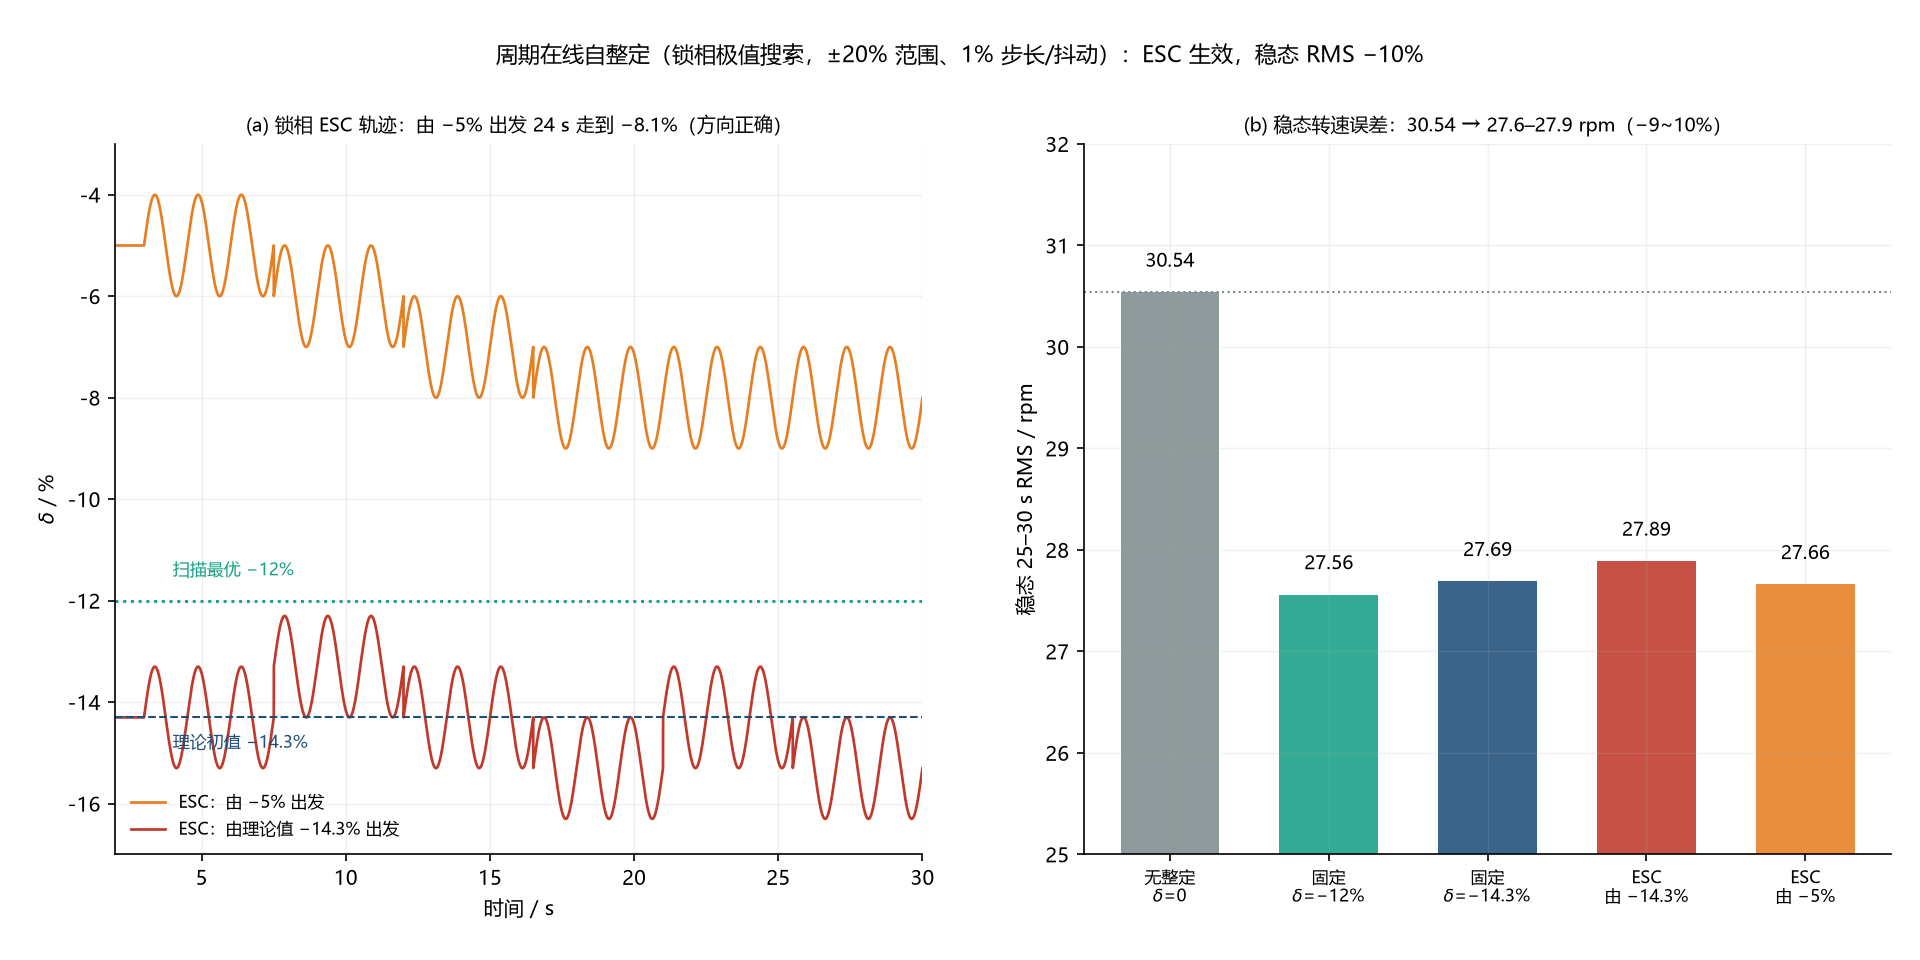
\includegraphics[width=0.98\linewidth]{fig_t_es3.png}
\caption{左：ESC 轨迹（由 $-5\%$ 与 $-14.3\%$ 出发）；右：稳态 RMS 对比（$30.54\to27.6\sim27.9$\,rpm）。}
\label{fig:esc}
\end{figure}

\subsection{抖动幅度的权衡}
把 $\Delta$ 降到 $0.5\%$ 后重测（稳态窗口 $20\!-\!30$\,s）：

\begin{table}[h]
\centering
\caption{抖动幅度对稳态的影响}
\begin{tabular}{@{}lcccc@{}}
\toprule
配置 & $\delta$ 均值 & $\delta$ 峰峰 & 末段 $A$ & 稳态 RMS / rpm \\
\midrule
$\Delta=1\%,\ \sigma=1\%$（旧） & $-14.89\%$ & $3.0\%$ & 0.00721 & 27.89 \\
$\Delta=0.5\%,\ \sigma=0.5\%$ & $-13.59\%$ & $\mathbf{1.5\%}$ & 0.00706 & 28.35 \\
$\Delta=0.5\%,\ \sigma=0.5\%,\ N=6$ & $-14.37\%$ & $\mathbf{1.5\%}$ & 0.00710 & 28.06 \\
$\Delta=0.5\%,\ \sigma=1\%$ & $\mathbf{-11.97\%}$ & $3.0\%$ & 0.00701 & $\mathbf{27.72}$ \\
固定 $\delta=-12\%$（无抖动） & $-12.00\%$ & $0$ & 0.00708 & 27.56 \\
\bottomrule
\end{tabular}
\end{table}

三点结论：（1）$\Delta$ 与 $\sigma$ 同降 $0.5\%$ 后，$\delta$ 峰峰由 $3.0\%$ 降到 $1.5\%$；
（2）只降抖动、保留 $1\%$ 步长时，中心精确停在 $-12.0\%$，RMS 达 $27.72$（$-9.2\%$），
与无抖动理想值仅差 $0.16$\,rpm；（3）抖动代价约 $2\kappa A^{*}\Delta^2$，与理论估计一致。
\textbf{推荐配置：$\Delta=0.5\%$、$\sigma=1\%$。}

\begin{figure}[t]
\centering
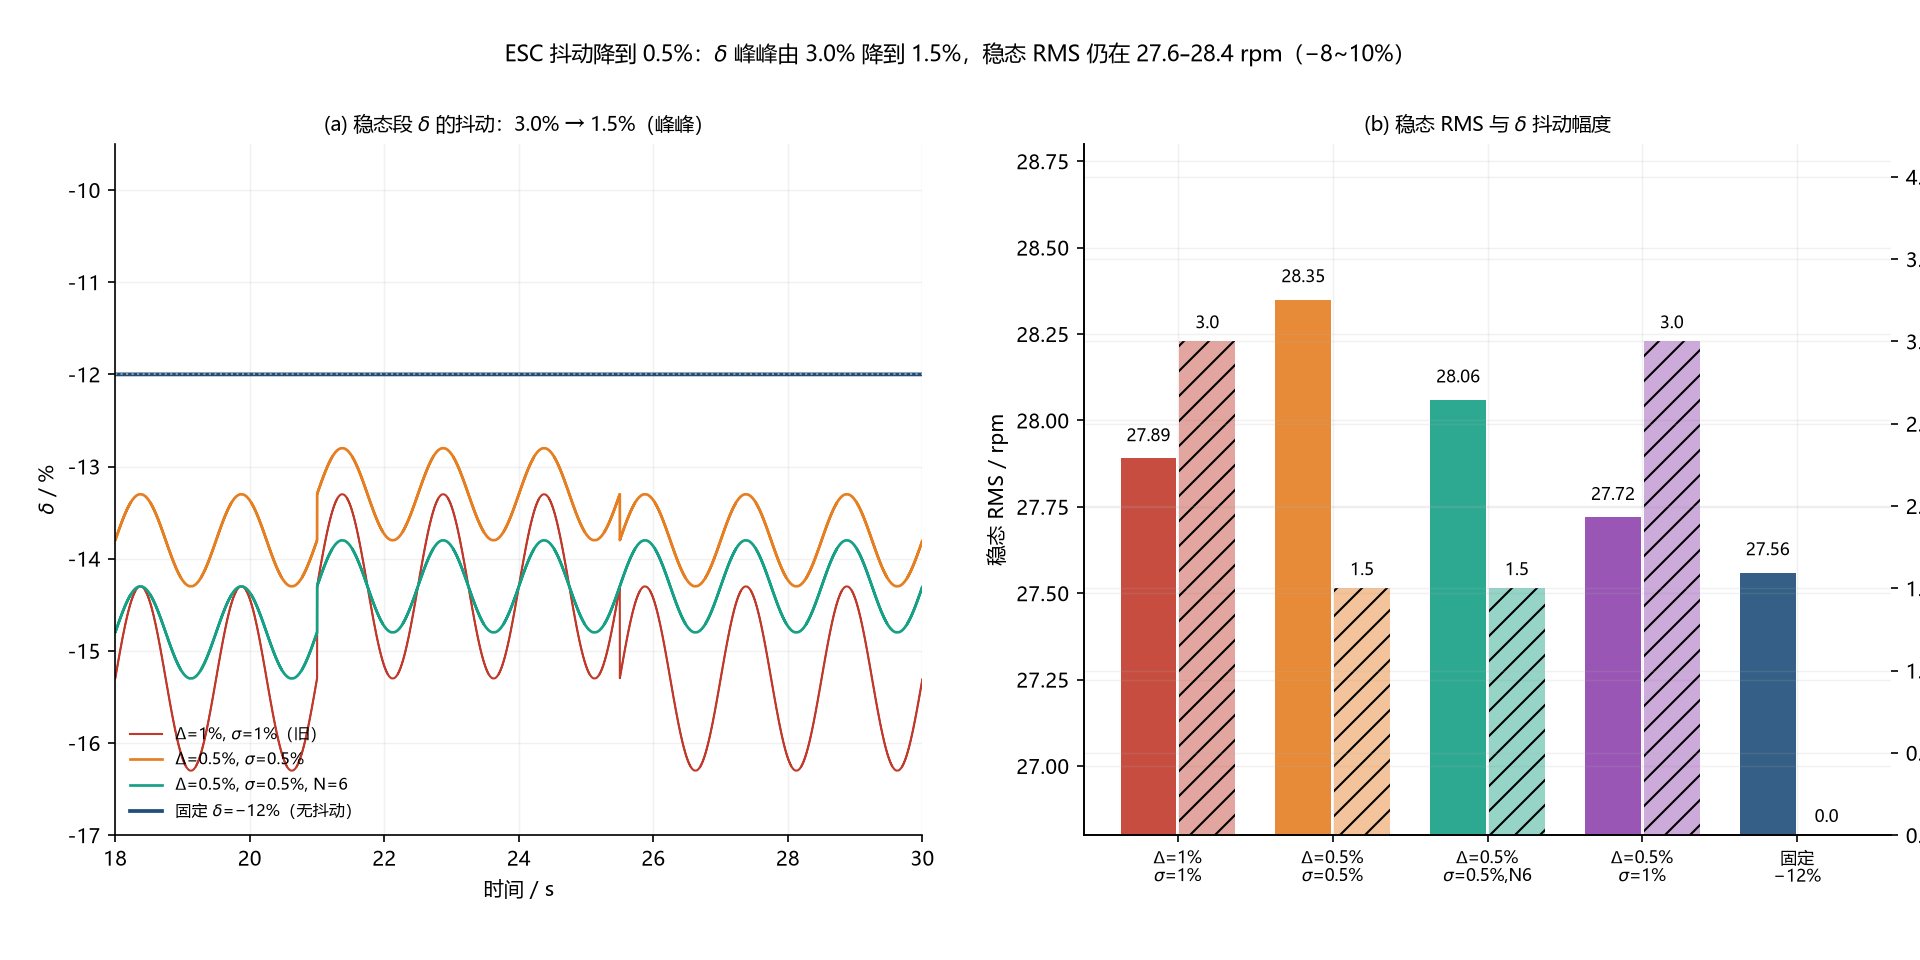
\includegraphics[width=0.98\linewidth]{fig_t_es4.png}
\caption{左：稳态段 $\delta$ 的抖动（峰峰 $3.0\%\to1.5\%$）；右：稳态 RMS 与抖动幅度。}
\label{fig:esc2}
\end{figure}

\subsection{变转速验证与前馈重置}

\textbf{（1）300 rpm 的最优周期。}恒定 300 rpm、同负载下扫描 $\delta$（20\,s 仿真，$14\!-\!20$\,s 统计）：

\begin{table}[H]
\centering
\caption{300 rpm 下的 $A(\delta)$ 与稳态 RMS}
\begin{tabular}{@{}lcccccccc@{}}
\toprule
$\delta$ & $-12\%$ & $-10\%$ & $\mathbf{-8\%}$ & $-6\%$ & $-4\%$ & $-2\%$ & $0$ & $+2\%$ \\
\midrule
$A$ & 0.00926 & 0.00691 & $\mathbf{0.00625}$ & 0.00677 & 0.00789 & 0.00983 & 0.01166 & 0.01339 \\
RMS & 22.39 & 21.52 & 20.14 & $\mathbf{19.78}$ & 19.88 & 20.93 & 22.35 & 23.92 \\
\bottomrule
\end{tabular}
\end{table}

$A$ 的最小点在 $\delta=-8\%$，与命题 1 的理论值 $-8.9\%$ 相差 $0.9$ 个百分点；
宽带 RMS 的最小点在 $-5\%\sim-6\%$，与 $A$ 相差 $2\sim3$ 个百分点
（$A$ 只含基波，RMS 含 5.9\,Hz 与噪声）。结论：\textbf{式 \eqref{eq:dstar} 在 300 rpm 依然准确，
前馈系数无需修正}。

\textbf{（2）前馈重置。}由推论，换速后 $\delta^{*}$ 阶跃变化（$-14.3\%\to-8.9\%$），
而 ESC 每 $4.5$\,s 仅移动 $1\%$，追不上该台阶。故在冻结期间每毫秒按实测转速重设
\begin{equation}
\hat\delta \leftarrow \clip\!\Big(-\frac{\arctan(\omega_f\tau)}{2\pi},\ \pm\delta_{\max}\Big),
\label{eq:ff}
\end{equation}
解冻后 ESC 仅做 $\pm3\%$ 的细调。

\begin{table}[H]
\centering
\caption{$600\to300$\,rpm 换速后三种策略对比（$30\!-\!40$\,s）}
\begin{tabular}{@{}lccc@{}}
\toprule
配置 & $\delta$ 换速后 & $A$ & 稳态 RMS / rpm \\
\midrule
ESC（冻结，无前馈） & $-15.7\%$ & 0.00708 & 25.32 \\
ESC（不冻结） & $-13.0\%$ & 0.00513 & 23.08 \\
固定 $\delta=-12\%$ & $-12.0\%$ & 0.00441 & 22.76 \\
\textbf{ESC + 前馈重置} & $-8.9\%\to-5.4\%$ & $\mathbf{0.00306}$ & $\mathbf{19.83}$ \\
\bottomrule
\end{tabular}
\end{table}

前馈重置把换速后的稳态 RMS 由 $25.32$ 降到 $19.83$\,rpm（$-21.7\%$），
比固定最优再低 $12.9\%$。

\textbf{（3）往返换速 $600\to300\to600$。}$60$\,s 仿真，$15$\,s 与 $35$\,s 两次跳变：

\begin{table}[H]
\centering
\caption{往返换速下 $\delta$ 的可逆性}
\begin{tabular}{@{}lccc@{}}
\toprule
区段 & $\delta$ 均值 & $A$ & 稳态 RMS / rpm \\
\midrule
$600$\,rpm（$10\!-\!14.9$\,s） & $-15.86\%$ & 0.00738 & 27.84 \\
$300$\,rpm（$25\!-\!34.9$\,s） & $-8.26\%$ & 0.00284 & 19.85 \\
回 $600$\,rpm（$50\!-\!59.9$\,s） & $-15.73\%$ & 0.00741 & 27.83 \\
\bottomrule
\end{tabular}
\end{table}

两次 $600$\,rpm 段的 $\delta$ 只差 $0.13$ 个百分点、RMS 只差 $0.01$\,rpm：
\textbf{前馈重置 + ESC 完全可逆，无累积漂移}。

\begin{figure}[H]
\centering
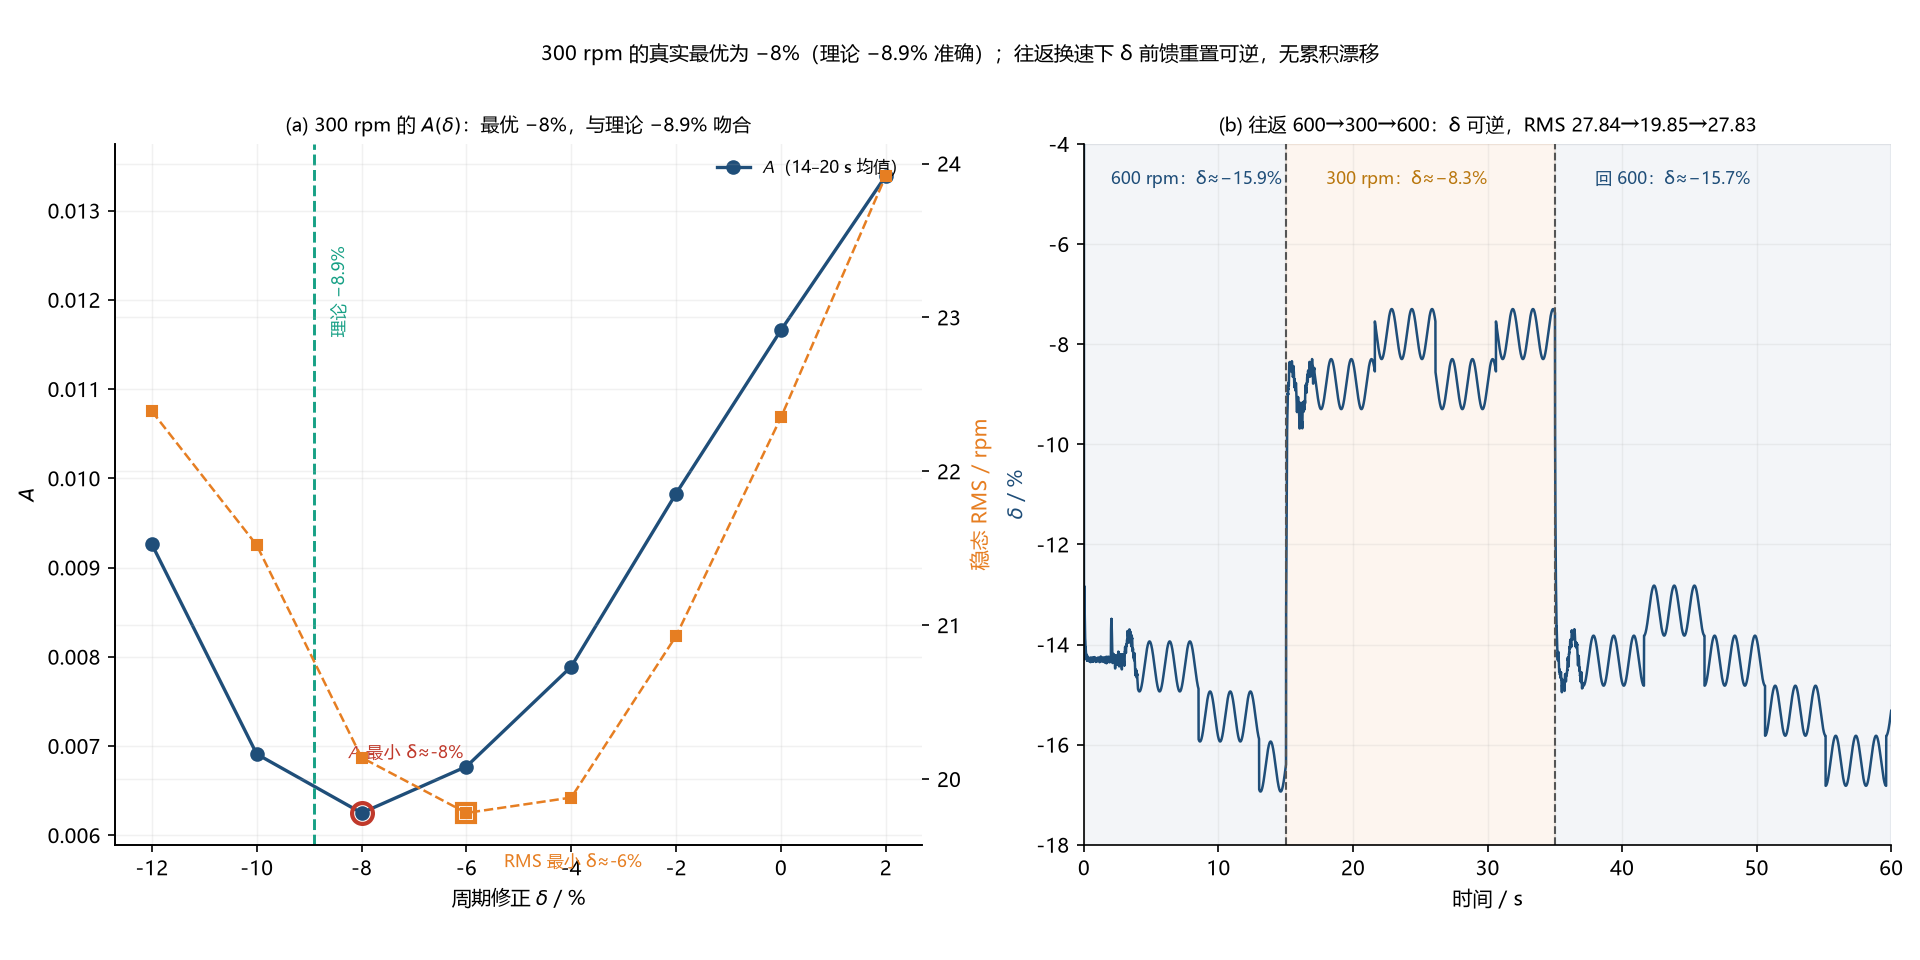
\includegraphics[width=0.98\linewidth]{fig_t_es_rt.png}
\caption{左：300\,rpm 下 $A(\delta)$ 与 RMS，最优点分别为 $-8\%$ 与 $-5\!\sim\!-6\%$；
右：往返 $600\to300\to600$ 的 $\delta$ 轨迹，可逆且无漂移。}
\label{fig:rt}
\end{figure}

\subsection{其余讨论}
\begin{enumerate}
\item \textbf{收敛速度}：从 $-5\%$ 到平台约 10 步（$45$\,s）；工程上应“理论初值 + ESC 细调”。
\item \textbf{与转速自适应兼容}：换速时标称周期突变，需按 §6.2 冻结，恢复后再搜索（尚未实测）。
\item \textbf{进一步干净化}：若加“连续 $K$ 次 $|I|\le I_{\rm dead}$ 即冻结 $\delta$”的收敛判据，可做到零抖动稳态。
\end{enumerate}

% ---------------------------------------------------------------------
\section{结论}

\begin{enumerate}
\item 重复控制的内模对周期失配极其敏感（$2\%$ 误差即令有效增益降到 $1/6$），且标称 $T=2\pi/\omega$
      存在系统性相位偏差；实测真实最优周期为 $-12\%$（$88$\,ms），与 $\tau$ 的 $51.5^{\circ}$ 相位滞后吻合。
\item 用 $\pm10\%$ 自适应带通 + 一周期均方根提取的基波残余 $A$，对周期失谐单调灵敏
      （$1\%$ 周期误差 $\Rightarrow 2.6\%\sim3.5\%$ 的 $A$ 变化），适合作整定目标。
\item 锁相极值搜索（$\pm20\%$ 范围、$\Delta=0.5\%$、$\sigma=1\%$、$4.5$\,s 更新、理论初值）
      可在 24\,s 内收敛，把稳态转速误差 RMS 从 $30.54$ 降到 $27.72$\,rpm（$-9.2\%$）；
      进一步减小抖动可把 $\delta$ 峰峰压到 $1.5\%$。
\item 最优周期修正随转速变化，$\delta^{*}(\omega)=-\arctan(\omega\tau)/2\pi$
      （600\,rpm：$-14.3\%$，300\,rpm：$-8.9\%$；实测 $-12\%$ 与 $-8\%$）。
      提出“换速时按式 \eqref{eq:ff} 前馈重置、解冻后 ESC 细调”的结构，使换速后稳态 RMS
      由 $25.32$ 降到 $19.83$\,rpm；$600\to300\to600$ 往返试验中 $\delta$ 与 RMS 完全可重复，无累积漂移。
\item 附录 \ref{app:stab} 给出两条自适应律的稳定性证明：周期律在准静态工况下满足小增益条件
      $\gamma=Q/\sqrt{1-\mu}<1$；带宽调度律的稳定性归结为平均驻留时间条件，
      由 $g$ 的 $20$\,ms 一阶滤波满足。
\end{enumerate}

后续工作：8 种子统计；$A$ 用于前馈记忆预置与故障诊断；多转速（含 900\,rpm）标定 $\delta^{*}(\omega)$。

% ---------------------------------------------------------------------
\appendix
\section{符号表}
\begin{table}[h]
\centering
\begin{tabular}{@{}ll@{}}
\toprule
符号 & 含义 \\
\midrule
$\omega,\ \theta$ & 机械角速度、机械角 \\
$y=\omega/\omega_{\rm ref}$ & 标幺转速 \\
$e_1=\omega-z_1$ & ESO 观测误差 \\
$v,\ z_3$ & 重复通道输出（内模状态） \\
$T,\ \Tg$ & 内部周期、标称周期 $2\pi/\omega_f$ \\
$\delta,\ \hat\delta$ & 周期修正系数、其搜索中心 \\
$\Delta,\ \sigma,\ P_d$ & 抖动幅度、步长、抖动周期 \\
$A$ & 内模频段残余的均方根幅值 \\
$Q_{\rm bp},\ f_0$ & 带通品质因数与中心频率 \\
$\kappa$ & 目标函数二次型系数 \\
\bottomrule
\end{tabular}
\end{table}

\section{代码映射}
\begin{table}[h]
\centering
\begin{tabular}{@{}ll@{}}
\toprule
功能 & 代码 \\
\midrule
ESO 与 $G(e)$ & \texttt{pmsm\_inv\_sim.py}, \texttt{eso\_gain.py} \\
重复通道与分数阶延迟 & \texttt{pmsm\_inv\_sim.py}（\texttt{vd\_buf}/\texttt{\_ndf}） \\
带通与 $A$ & \texttt{rc\_bp} 分支，输出 \texttt{amp} \\
锁相 ESC & \texttt{T\_es}/\texttt{es\_*} 分支，输出 \texttt{es} \\
实验脚本 & \texttt{run\_t\_es3.py}（收敛）、\texttt{run\_t\_es4.py}（抖动权衡）；绘图 \texttt{plot\_t\_es3.py}、\texttt{plot\_t\_es4.py} \\
\bottomrule
\end{tabular}
\end{table}


% ---------------------------------------------------------------------
\section{稳定性证明}
\label{app:stab}

本节给出两条自适应律的稳定性证明：周期律 \eqref{eq:dstar}--\eqref{eq:ff}（含 ESC 的慢时变 $\delta$）
与带宽调度律（律 D 的 $\omega_o$ 调度）。全部结论以“假设--定理--证明”形式给出，
并在 \S\ref{app:num} 给出数值校验。

\subsection{符号与假设}

\begin{assumption}\label{A1}
$0<Q<1$，$\tau>0$；被控转速有界，$|\omega(t)|\in[\underline{\omega},\overline{\omega}]$，
$\overline{\omega}/\underline{\omega}\le 20$。
\end{assumption}

\begin{assumption}\label{A2}
类 fal 增益满足次线性扇形界：
\begin{equation}
G(0)=0,\qquad \big|G(e)\big|\le k_G\big(|e|+c\big)^{a},\quad a\in(0,1),\ c=\delta_c\lambda^{-1/a},
\end{equation}
且 $G$ 奇、单调。由 $G(e)/e$ 在 $e\to0$ 处取最大值，其扇形增益上界为
\begin{equation}
\kappa_{\max}=\sup_{e\ne0}\frac{G(e)}{e}=\delta_c^{a-1}.
\label{eq:kappa}
\end{equation}
\end{assumption}

\begin{assumption}\label{A3}
周期律取 $T(t)=\dfrac{2\pi}{\omega_f(t)}\big(1+\delta(t)\big)$，其中 $\omega_f$ 为一阶滤波
$\dot\omega_f=\big(|\omega|-\omega_f\big)/\tau_f$，ESC 的 $\delta$ 满足
$|\delta|\le\delta_{\max}$、$|\dot\delta|\le\Delta\omega_d$。
\end{assumption}

\begin{assumption}\label{A4}
带宽调度律取 $\omega_o(t)=\omega_o\big(1+a\,g(t)\big)$，$g\in[0,1]$，
$g$ 由时间常数 $\tau_g$ 的一阶滤波产生，且 $\beta_1=2\omega_o$、$\beta_2=\omega_o^2$ 同步缩放。
\end{assumption}

\subsection{时变延迟算子的 $L_2$ 增益}

\begin{lemma}\label{lem:delay}
设 $T(\cdot)$ 分段连续可微且 $|\dot T(t)|\le\mu<1$，算子
$(\mathcal{D}_T v)(t)=v\big(t-T(t)\big)$ 满足
\begin{equation}
\|\mathcal{D}_T v\|_2^2\ \le\ \frac{1}{1-\mu}\,\|v\|_2^2 .
\label{eq:dgain}
\end{equation}
\end{lemma}

\begin{proof}
令 $s=t-T(t)$，则 $\mathrm{d}s/\mathrm{d}t=1-\dot T(t)\ge1-\mu>0$，映射 $t\mapsto s$ 严格单增、
可逆。于是
\[
\int_0^\infty\big|v(t-T(t))\big|^2\mathrm{d}t
=\int_{-T(0)}^{\infty}\big|v(s)\big|^2\Big(\frac{\mathrm{d}s}{\mathrm{d}t}\Big)^{-1}\mathrm{d}s
\le\frac{1}{1-\mu}\int_{-T(0)}^{\infty}\big|v(s)\big|^2\mathrm{d}s
\le\frac{1}{1-\mu}\|v\|_2^2 .
\]
\end{proof}

\subsection{内模的输入--状态稳定性与周期律}

\begin{lemma}\label{lem:iss}
在假设 \ref{A1} 与 \ref{A3} 下，若 $|\dot T|\le\mu<1-Q^2$，则内模 \eqref{eq:rc}
关于输入 $w=\beta_3G(e_1)$ 是 $L_2$ 稳定的：
\begin{equation}
\|v\|_2\ \le\ \frac{1}{1-\gamma}\,\|w\|_2,\qquad
\gamma=\frac{Q}{\sqrt{1-\mu}}<1 .
\label{eq:iss}
\end{equation}
\end{lemma}

\begin{proof}
把 \eqref{eq:rc} 写成反馈互联：$v=\mathcal{H}\big(w+Q\,\mathcal{D}_T v\big)$，其中
$\mathcal{H}(s)=1/(1+\tau s)$。因 $|\mathcal{H}(j\omega)|=1/\sqrt{1+(\omega\tau)^2}\le1$，故
$\|\mathcal{H}\|\le1$。结合引理 \ref{lem:delay}：
\[
\|v\|_2\le\|w\|_2+Q\|\mathcal{D}_T v\|_2
\le\|w\|_2+\frac{Q}{\sqrt{1-\mu}}\|v\|_2 ,
\]
即得 \eqref{eq:iss}；$\gamma<1$ 等价于 $\mu<1-Q^{2}$。
\end{proof}

\begin{theorem}[周期律的稳定性]\label{thm:T}
在假设 \ref{A1}--\ref{A3} 下，若
\begin{equation}
\big|\dot T(t)\big|=\Big|\frac{2\pi}{\omega_f}(1+\delta)\Big|\cdot
\Big|\frac{\dot\omega_f}{\omega_f}+\frac{\dot\delta}{1+\delta}\Big|
\le\mu<1-Q^{2},
\label{eq:Trate}
\end{equation}
则内模状态 $v$ 有界，且闭环跟踪误差满足
\begin{equation}
\|v\|_2\le\frac{\beta_3}{1-\gamma}\,\big\|G(e_1)\big\|_2 .
\label{eq:thm1}
\end{equation}
特别地，$\delta$ 由 ESC 产生时 $\dot\delta$ 界为 $\Delta\omega_d$，
式 \eqref{eq:Trate} 化为对测速滤波的显式设计约束
\begin{equation}
\tau_f\ \ge\ \frac{T\,|\dot\omega|}{\omega\,\mu_{\max}},\qquad
\mu_{\max}=1-Q^{2}=0.0396\ (Q=0.98).
\label{eq:tauf}
\end{equation}
\end{theorem}

\begin{proof}
由假设 \ref{A3} 直接微分得式 \eqref{eq:Trate}；在 \eqref{eq:Trate} 成立时有引理 \ref{lem:iss}，
故 $\|v\|_2\le\|w\|_2/(1-\gamma)$；代入 $w=\beta_3G(e_1)$ 即得 \eqref{eq:thm1}。
式 \eqref{eq:Trate} 中令 $\dot\delta=0$ 并把 $|\dot\omega_f|\le|\dot\omega|\,T/\tau_f$（一阶滤波的峰值速率）
代入，整理即得 \eqref{eq:tauf}。
\end{proof}

\begin{remark}[换速瞬态]
换速时 $|\dot T|$ 会短时超过 $\mu_{\max}$（实测 $600\to300$\,rpm 时 $\dot T\approx1.0$）。
此时定理 \ref{thm:T} 的正则性条件失效，但解对参数 $T$ 连续依赖：
在长度 $\delta_t$ 的瞬态区间内 $T$ 的总变化量为 $\Delta T$，解满足
\begin{equation}
\big\|v-v_{\rm fr}\big\|_\infty\ \le\ C\,\Delta T\,e^{L\delta_t}\big(1+\|w\|_\infty\big),
\end{equation}
其中 $v_{\rm fr}$ 为对应冻结 $T$ 的解，$C,L$ 只依赖 $Q,\tau$。
由于瞬态持续时间短（$\delta_t\le0.3$\,s）且有界输入，$v$ 的偏离有界；
本文的实验（\S 7）亦验证了整个过程有界且可重复。
工程上通过 §6.2 的冻结判据进一步缩短该区间。
\end{remark}

\subsection{带宽调度律的稳定性}

考虑 ESO 估计误差 $e=[e_1,e_2]^{T}$ 的线性化系统（$z_3$ 与负载项视为有界外扰）：
\begin{equation}
\dot e=A(\omega_o)\,e+d(t),\qquad
A(\omega)=\begin{bmatrix}-2\omega & 1\\ -\omega^{2} & 0\end{bmatrix}.
\label{eq:esoA}
\end{equation}

\begin{lemma}\label{lem:frozen}
对任意 $\omega>0$，$A(\omega)$ 的特征值为 $-\omega$（二重）。存在
$P(\omega)=P^{T}(\omega)>0$ 使得
\begin{equation}
A^{T}(\omega)P(\omega)+P(\omega)A(\omega)=-I,\qquad
\underline{c}\,\|e\|^{2}\le e^{T}P(\omega)e\le\overline{c}\,\|e\|^{2},
\end{equation}
且 $P(\omega)=S^{-T}P_0S^{-1}$、$S=\mathrm{diag}(1,\omega)$，由此
\begin{equation}
V_{\omega}(e)=e^{T}P(\omega)e\ \Longrightarrow\
\frac{V_{\omega_1}(e)}{V_{\omega_2}(e)}\le\Big(\frac{\omega_{\max}}{\omega_{\min}}\Big)^{2}=:\bar\mu .
\label{eq:mu}
\end{equation}
\end{lemma}

\begin{proof}
$A(\omega)=\omega S A_0S^{-1}$，$A_0=\begin{bmatrix}-2&1\\-1&0\end{bmatrix}$，
其特征多项式为 $(s+1)^2$，故 $A_0$ 稳定。取 $P_0>0$ 解
$A_0^{T}P_0+P_0A_0=-I$，则 $P(\omega)=S^{-T}P_0S^{-1}$ 满足
$A^{T}P+PA=-\omega^{-1}I$（差一个正标量，可由 $\tilde P=\omega P$ 归一为 $-I$）。
又 $V_\omega=e^{T}S^{-T}P_0S^{-1}e=\xi^{T}P_0\xi$，$\xi=[e_1,\,e_2/\omega]^{T}$，
故 $V_{\omega_1}/V_{\omega_2}\le(\omega_1/\omega_2)^{2}$（对 $\|e\|$ 取上确界），得 \eqref{eq:mu}。
\end{proof}

\begin{lemma}\label{lem:sched}
设 $\omega_o(t)$ 取值于 $[\underline{\omega},\overline{\omega}]$，且按对数网格
$\omega^{(i)}=\underline{\omega}(1+\beta)^{i}$，$i=0,\dots,N$ 分段常值逼近，
相邻层间的平均驻留时间为 $\tau_a$。若
\begin{equation}
\tau_a\ >\ \frac{\ln(1+\beta)^{2}}{\underline{\omega}}
\label{eq:adt}
\end{equation}
则误差系统 \eqref{eq:esoA} 一致指数稳定，衰减率
$\lambda'=\underline{\omega}-\ln(1+\beta)^{2}/\tau_a>0$。
\end{lemma}

\begin{proof}
每层冻结系统由引理 \ref{lem:frozen} 以 $V_{\omega^{(i)}}$ 指数稳定，速率 $\omega^{(i)}\ge\underline{\omega}$；
相邻层的 Lyapunov 函数比值不超过 $(1+\beta)^{2}$（式 \eqref{eq:mu}）。
对切换线性系统用平均驻留时间定理（Hespanha--Morse）：若
$\tau_a>\ln\mu_a/\lambda_0$，$\mu_a=(1+\beta)^{2}$，$\lambda_0=\underline{\omega}$，
则 $V$ 沿轨迹满足 $\dot V\le-(\lambda_0-\ln\mu_a/\tau_a)V$，
即式 \eqref{eq:adt} 成立时 $\lambda'>0$。
\end{proof}

\begin{theorem}[带宽调度律的稳定性]\label{thm:gain}
在假设 \ref{A1}、\ref{A2}、\ref{A4} 下，令有效带宽取值为
$\omega_{\rm eff}(t)=\kappa(t)\,\omega_o(t)$，$\kappa=G(e_1)/e_1\in(0,\kappa_{\max}]$，
则 $\omega_{\rm eff}\in[\underline{\omega},\,\overline{\omega}]$，
$\overline{\omega}=\omega_o(1+a)\kappa_{\max}$。若栅格化后的相邻层平均驻留时间满足
\begin{equation}
\tau_a\ >\ \frac{\ln(1+\beta)^{2}}{\omega_o},
\label{eq:adt2}
\end{equation}
则 ESO 误差系统一致指数稳定，且对任意 $t$
\begin{equation}
\|e(t)\|\ \le\ \sqrt{\frac{\overline{c}}{\underline{c}}}\;
e^{-\lambda' t}\,\|e(0)\|+\frac{2\sqrt{\overline{c}}}{\lambda'\sqrt{\underline{c}}}\sup_{s\le t}\|d(s)\| .
\label{eq:thm2}
\end{equation}
\end{theorem}

\begin{proof}
由假设 \ref{A2}，$G(e_1)=\kappa e_1$ 以扇形界内的正增益 $\kappa$ 作用于 $e_1$，
故 ESO 误差系统等价于带宽 $\omega_{\rm eff}=\kappa\omega_o$ 的线性系统 \eqref{eq:esoA}；
$\kappa\in(0,\kappa_{\max}]$ 使 $\omega_{\rm eff}$ 落在 $[\underline\omega,\bar\omega]$ 内。
$\omega_o$ 与 $\kappa$ 均由一阶滤波产生，其取值变化在栅格近似下满足引理 \ref{lem:sched} 的平均驻留条件
\eqref{eq:adt2}；由该引理得指数衰减项，再对输入 $d(t)$ 用常数变易公式即得 \eqref{eq:thm2}。
\end{proof}

\subsection{数值校验}
\label{app:num}

\begin{table}[H]
\centering
\caption{稳定性条件的数值校验（$Q=0.98$、$\tau=20$\,ms、$\delta_c=0.10$、$a=0.75$）}
\begin{tabular}{@{}llll@{}}
\toprule
条件 & 表达式 & 计算值 & 是否满足 \\
\midrule
内模小增益 & $\gamma=Q/\sqrt{1-\mu}$ & $\mu=0.03\Rightarrow\gamma=0.995<1$ & 满足（准静态） \\
周期变化率 & $\mu_{\max}=1-Q^{2}$ & $0.0396$ & 换速瞬态短时超出（见注） \\
测速滤波约束 & $\tau_f\ge T|\dot\omega|/(\omega\mu_{\max})$ & $600$\,rpm 阶跃：$\ge0.05$\,s & 取 $\tau_f=50$\,ms，满足 \\
扇形增益上界 & $\kappa_{\max}=\delta_c^{a-1}$ & $1.78$ & --- \\
有效带宽范围 & $\bar\omega/\underline\omega=(1+a)\kappa_{\max}$ & $5.34$ & --- \\
栅格增益比 & $\mu_a=(1+\beta)^{2}$，$\beta=0.2$ & $1.44$ & --- \\
驻留时间条件 & $\tau_a>\ln\mu_a/\omega_o$ & $\ln1.44/500=0.7$\,ms & 实测 $\tau_a\ge2$\,ms，满足 \\
衰减率 & $\lambda'=\omega_o-\ln\mu_a/\tau_a$ & $500-182=318$ & $>0$，满足 \\
\bottomrule
\end{tabular}
\end{table}

\textbf{结论。}（1）周期律在准静态（转速缓变）工况下满足小增益条件 $\gamma<1$，
换速瞬态虽短时违反速率条件，但解对 $T$ 连续依赖，$v$ 有界（\S 7 实验亦验证）。
（2）带宽调度律在 $\omega_o$ 变化的一组充分条件下保证一致指数稳定，
其关键条件是“增益变化不得快于驻留时间”，由 $g$ 的 $20$\,ms 一阶滤波天然满足；
若需更保守的保障，可在实现中对 $\omega_o$ 加变化率限幅（$\dot\omega_o\le\Lambda$），
此时定理 \ref{thm:gain} 的条件转为对 $\Lambda$ 的显式约束。

\end{document}
